\documentclass[tikz,border=12pt]{standalone}
\usepackage[T1]{fontenc}
\usepackage{helvet}
\renewcommand{\familydefault}{\sfdefault}
\usepackage{amsmath}
\usetikzlibrary{arrows.meta, fit, backgrounds, positioning, calc, shapes.geometric}

% Semantic palette, shared across the method figures. Color encodes role:
%   blue   = BM25 / lexical step
%   red    = LLM step
%   amber  = document data and stores
%   green  = retrieved units and final output (leaves, candidates, passages)
%   gray   = query input and neutral combine step
\definecolor{queryfill}{HTML}{ECEFF2}
\definecolor{queryborder}{HTML}{8A96A3}
\definecolor{bm25fill}{HTML}{E2ECF7}
\definecolor{bm25border}{HTML}{3C6CA6}
\definecolor{llmfill}{HTML}{F7E4E4}
\definecolor{llmborder}{HTML}{BE4F4F}
\definecolor{corpusfill}{HTML}{FBF0D5}
\definecolor{corpusborder}{HTML}{CFA23E}
\definecolor{outfill}{HTML}{E7F4E7}
\definecolor{outborder}{HTML}{59A05B}
\definecolor{poolfill}{HTML}{F1F9F1}
\definecolor{regfill}{HTML}{F6F8FB}
\definecolor{regborder}{HTML}{C4CDD6}
\definecolor{darkline}{HTML}{333333}
\definecolor{subtext}{HTML}{5A5A5A}

\tikzset{
  card/.style={rectangle, rounded corners=5pt, align=center, draw=darkline,
               line width=0.8pt, minimum height=1.1cm, font=\small},
  query/.style={card, fill=queryfill, draw=queryborder, minimum width=2.0cm},
  proc/.style={card, fill=bm25fill, draw=bm25border, minimum width=2.4cm},
  llmproc/.style={card, fill=llmfill, draw=llmborder, minimum width=2.4cm},
  mrg/.style={card, fill=queryfill, draw=queryborder, minimum width=2.1cm},
  result/.style={card, fill=outfill, draw=outborder, minimum width=2.1cm},
  leaf/.style={rectangle, rounded corners=3pt, draw=outborder, fill=outfill,
               line width=0.8pt, minimum width=1.05cm, minimum height=0.8cm, font=\scriptsize},
  db/.style={cylinder, shape border rotate=90, aspect=0.28, draw=corpusborder,
             fill=corpusfill, line width=0.8pt, minimum width=1.7cm,
             minimum height=1.0cm, font=\scriptsize, align=center, inner sep=1pt},
  region/.style={rounded corners=12pt, fill=regfill, draw=regborder, line width=0.8pt},
  pooldash/.style={draw=outborder, dashed, rounded corners=8pt, fill=poolfill,
                   line width=0.85pt},
  regtitle/.style={font=\small\bfseries, text=darkline},
  note/.style={font=\scriptsize\itshape, text=subtext, align=center},
  flow/.style={-{Latex[length=2.2mm]}, line width=0.85pt, draw=darkline},
  feed/.style={-{Latex[length=1.9mm]}, line width=0.7pt, draw=corpusborder},
}

\def\cspread{0.95cm}

\begin{document}
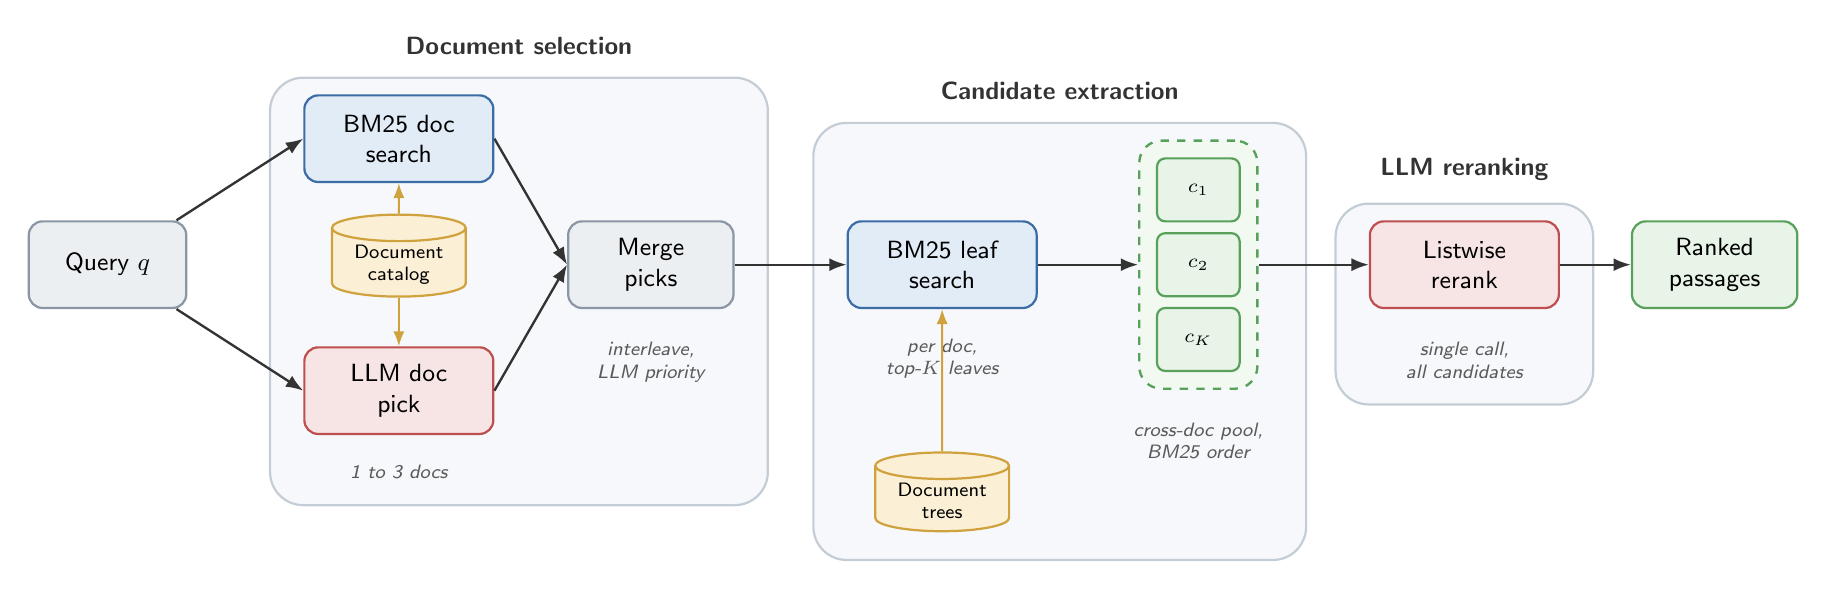
\begin{tikzpicture}

% Input (outside the phases)
\node[query] (query) at (0.3,0) {Query $q$};

% Stage 1: hybrid document selection. The catalog sits in the gap between the
% two picks and feeds straight up and straight down, so its arrows are short
% verticals that never tangle with the query fan arriving from the left.
\node[proc]    (bm25doc) at (4.0, 1.6)  {BM25 doc\\search};
\node[llmproc] (llmdoc)  at (4.0,-1.6)  {LLM doc\\pick};
\node[db]      (catalog) at (4.0, 0)    {Document\\catalog};
\node[mrg]     (merge)   at (7.2, 0)    {Merge\\picks};

% Stage 2: per-document BM25 leaf candidates, pooled cross-document
\node[proc] (bm25leaf) at (10.9, 0)   {BM25 leaf\\search};
\node[db]   (trees)    at (10.9,-3.0) {Document\\trees};
\node[leaf, right=1.5cm of bm25leaf, yshift=\cspread]  (c1) {$c_1$};
\node[leaf, right=1.5cm of bm25leaf]                   (c2) {$c_2$};
\node[leaf, right=1.5cm of bm25leaf, yshift=-\cspread] (ck) {$c_K$};
\node[font=\footnotesize] at ($(c2)!0.5!(ck)$) {$\vdots$};
\node[pooldash, fit=(c1)(c2)(ck), inner sep=6pt] (cpool) {};
\foreach \n/\t in {c1/c_1, c2/c_2, ck/c_K} { \node[leaf] at (\n) {$\t$}; }

% Stage 3: single cross-document LLM listwise rerank
\node[llmproc, right=1.4cm of cpool] (rerank) {Listwise\\rerank};

% Output (outside the phases)
\node[result, right=0.9cm of rerank] (sources) {Ranked\\passages};

% Notes
\node[note, below=0.26cm of llmdoc] (llmdocnote) {1 to 3 docs};
\node[note, below=0.30cm of merge] (mergenote) {interleave,\\LLM priority};
\node[note, below=0.26cm of bm25leaf] (leafnote) {per doc,\\top-$K$ leaves};
\node[note, below=0.30cm of cpool] (candnote) {cross-doc pool,\\BM25 order};
\node[note, below=0.30cm of rerank] (reranknote) {single call,\\all candidates};

% Phase panels. Input and output stay outside.
\begin{scope}[on background layer]
  \coordinate (bandB) at ($(trees.south)+(0,-0.14)$);
  \node[region, inner xsep=12pt, inner ysep=6pt,
        fit=(bm25doc)(llmdoc)(llmdocnote)(catalog)(merge)(mergenote)] (reg1) {};
  \node[region, inner xsep=12pt, inner ysep=6pt,
        fit=(bm25leaf)(leafnote)(trees)(cpool)(candnote)(bm25leaf|-bandB)] (reg2) {};
  \node[region, inner xsep=12pt, inner ysep=6pt,
        fit=(rerank)(reranknote)] (reg3) {};
\end{scope}
\node[regtitle, anchor=south] at ($(reg1.north)+(0,0.16)$) {Document selection};
\node[regtitle, anchor=south] at ($(reg2.north)+(0,0.16)$) {Candidate extraction};
\node[regtitle, anchor=south] at ($(reg3.north)+(0,0.16)$) {LLM reranking};

% Flow
\draw[flow] (query) -- (bm25doc.west);
\draw[flow] (query) -- (llmdoc.west);
\draw[feed] (catalog.north) -- (bm25doc.south);
\draw[feed] (catalog.south) -- (llmdoc.north);
\draw[flow] (bm25doc.east) -- (merge.west);
\draw[flow] (llmdoc.east) -- (merge.west);
\draw[flow] (merge.east) -- (bm25leaf.west);
\draw[feed] (trees.north) -- (bm25leaf.south);
\draw[flow] (bm25leaf.east) -- (cpool.west);
\draw[flow] (cpool.east) -- (rerank.west);
\draw[flow] (rerank.east) -- (sources.west);

\end{tikzpicture}
\end{document}
